\clearpage
%\setcounter{page}{1}
\maketitlesupplementary

\section{Pre-training Objective}
\label{lbd}
The proposed DriveWorld for 4D driving pre-training encompasses the following five components:

%\vspace{-1em}
\begin{footnotesize} 
	\begin{equation} \label{world_model}
	\begin{aligned}
	{\rm BEV \, Representation \, Model:}\, &b_t\sim q_\phi  (b_t\mid o_t) \\
	{\rm Stochastic \, State \, Model:}\, &s_t\sim q_\phi  (s_t\mid h_{t},a_{t-1},o_t) \\
	{\rm Dynamic \, Transition \, Model:}\, &s_t\sim p_\theta (s_t\mid h_t,\hat{a}_{t-1}) \\
	{\rm Static \, Propagation \, Model:}\, &\hat{b}\sim p_\theta (\hat{b}\mid b^{'}) \\
	{\rm Action \, Decoder:}\, &\hat{a}_t\sim p_\theta  (\hat{a}_t\mid h_{t},s_t) \\
	{\rm 3D \, Occupancy \, Decoder:}\, &\hat{y}_t\sim p_\theta  (\hat{y}_t\mid h_{t},s_t,\hat{b}). \\
	\end{aligned}
	\end{equation} 
\end{footnotesize}

The joint probability distribution for DriveWorld is:

%\vspace{-1em}
\begin{footnotesize} 
	\begin{equation} \label{v1}
	\begin{aligned}
	&p(h_{1:T},s_{1:T},y_{1:T+L},a_{1:T+L})=\\&\displaystyle\prod_{t=1}^{T}p(h_t,s_t|h_{t-1},s_{t-1},a_{t-1})p(y_t,a_t|h_t,s_t,\hat{b})\\
	&\displaystyle\prod_{k=1}^{L}p(h_k,s_k|h_{T},s_{T},a_{k-1})p(y_k,a_k|h_T,s_T,\hat{b}),
	\end{aligned}
	\end{equation} 
\end{footnotesize}

with 

%\vspace{-1em}
\begin{footnotesize} 
	\begin{equation} \label{v21}
	p(h_t,s_t|h_{t-1},s_{t-1},a_{t-1})=p(h_t|h_{t-1},s_{t-1})p(s_t|h_t,a_{t-1}),
	\end{equation} 
\end{footnotesize}

%\vspace{-1em}
\begin{footnotesize} 
	\begin{equation} \label{v22}
	p(y_t,a_t|h_{t},s_{t})=p(y_t|h_{t},s_{t},\hat{b})p(a_t|h_t,s_{t}),
	\end{equation}
\end{footnotesize} 

%\vspace{-1em}
\begin{footnotesize} 
	\begin{equation} \label{v23}
	p(y_k,a_k|h_{T},s_{T})=p(y_k|h_{T},s_{T},\hat{b})p(a_{k}|h_T,s_{T}).
	\end{equation}
\end{footnotesize} 

Given that $h_t$ is deterministic~\cite{plas_wm,dreamerv2,mile}, we have $p(h_t|h_{t-1},s_{t-1})=\delta(h_t-f_\theta(\hat{h}_{t-1},\rm MLN(s_{t-1})))$. Consequently, to maximize the marginal likelihood of $p(y_{1:{T+L}},a_{1:{T+L}})$, it is imperative to infer the latent variables $s_{1:T}$. This is achieved through deep variational inference, wherein we introduce a variational distribution $q_{H,S}$ defined and factorized as follows:

%\vspace{-1em}
\begin{footnotesize} 
	\begin{equation} \label{v3}
	\begin{aligned}
	q_{H,S}&\triangleq q(h_{1:T},s_{1:T}|o_{1:T},y_{1:T+L},a_{1:T+L})\\
	&=\displaystyle\prod_{t=1}^{T}q(h_t|h_{t-1},s_{t-1})q(s_t|o_{\le t},a_{< t}).
	\end{aligned}
	\end{equation} 
\end{footnotesize}

We parameterise this variational distribution with a neural network with weights $\phi $. By formalizing the above process as a generative probabilistic model, we can obtain a variational lower bound on the log evidence:

%\vspace{-1em}
\begin{footnotesize}
	\begin{equation} \label{vae}
	\begin{aligned}
	&{\rm log} p(y_{1:T+L},a_{1:T+L})\ge \mathcal{L}(y_{1:T+L},a_{1:T+L};\theta ,\phi ) \\ &\triangleq  \displaystyle\sum_{t=1}^{T}\mathbb{E}_{h_{1:t},s_{1:t}\backsim q(h_{1:t},s_{1:t}|o_{\leq t},a_{<t})}[\underbrace{\log p(y_t|h_t,s_t,\hat{b})}_{{\rm past \ occupancy\, loss}}\\
	&\qquad+\underbrace{\log p(a_t|h_t,s_t)}_{{\rm past \ action\, loss}}]  +\displaystyle\sum_{k=1}^{L}\mathbb{E}_{h_{T},s_{T}\backsim q(h_{T},s_{T}|o_{\leq T},a_{<T})}\\
	&\qquad[\underbrace{\log p(y_{T+k}|h_T,s_T,\hat{b})}_{{\rm future \ occupancy\, loss}}+\underbrace{\log p(a_{T+k}|h_T,s_T)}_{{\rm future \ action\, loss}}] \\
	&\quad-\displaystyle\sum_{t=1}^{T}\mathbb{E}_{h_{1:t-1},s_{1:t-1}\backsim q(h_{1:t-1},s_{1:t-1}|o_{\leq t-1},a_{<t-1} )}\\
	&\qquad[\underbrace{D_{KL}(q(s_t|o_{\leq t},a_{<t})\parallel p(s_t|h_{t-1},s_{t-1}))}_{{\rm posterior\, and\, prior\, matching\, KL\, loss}}].
	\end{aligned}
	\end{equation} 
\end{footnotesize}

In Eqn.~\ref{vae}, we model $q(s_t|o_{1:t}, a_{1:t-1})$ as a Gaussian distribution, allowing for the closed-form computation of the Kullback-Leibler (KL) divergence. The modelling of actions as a Laplace distribution and 3D occupancy labels as a categorical distribution results in L1 and cross-entropy losses, respectively. 
%\vspace{-1em}
\section{Lower Bound Derivation} 

Next, we will derive the variational lower bound in Eqn.~\ref{vae}. Let $q_{H,S}\triangleq q(h_{1:T},s_{1:T}|o_{1:T},y_{1:T+L},a_{1:T+L})$ be the variational distribution and $p(h_{1:T},s_{1:T}|a_{1:T+L},y_{1:T+L})$ be the posterior distribution. The Kullback-Leibler divergence between these two distributions is:

%\vspace{-1em}
\begin{footnotesize} 
	\begin{equation} \label{1}
	\begin{aligned}
	&D_{KL}(q(h_{1:T},s_{1:T}|o_{1:T},y_{1:T+L},a_{1:T+L})  \\
	&\quad \parallel p(h_{1:T},s_{1:T}|y_{1:T+L},a_{1:T+L}))\\
	&=\mathbb{E}_{h_{1:T},s_{1:T}\backsim q_{H,S}}[{\log}\tfrac{q(h_{1:T},s_{1:T}|o_{1:T},y_{1:T+L},a_{1:T+L})}{p(h_{1:T},s_{1:T}|y_{1:T+L},a_{1:T+L})}]\\
	&=\mathbb{E}_{h_{1:T},s_{1:T}\backsim q_{H,S}}\\
	&\quad[{\log}\tfrac{q(h_{1:T},s_{1:T}|o_{1:T},y_{1:T+L},a_{1:T+L})p(y_{1:T+L},a_{1:T+L})}{p(h_{1:T},s_{1:T})p(y_{1:T+L},a_{1:T+L}|h_{1:T},s_{1:T})}]\\  
	&=\log p(y_{1:T+L},a_{1:T+L})- \\
	&\quad \mathbb{E}_{h_{1:T},s_{1:T}\backsim q_{H,S}}[\log p(y_{1:T+L},a_{1:T+L}|h_{1:T},s_{1:T})]+ \\ 
	&\quad D_{KL}(q(h_{1:T},s_{1:T}|o_{1:T},y_{1:T+L},a_{1:T+L})\parallel p(h_{1:T},s_{1:T})).
	\end{aligned}
	\end{equation} 
\end{footnotesize}

Since $D_{KL}(q(h_{1:T},s_{1:T}|o_{1:T},y_{1:T+L},a_{1:T+L})\parallel p(h_{1:T},s_{1:T}|y_{1:T+L},a_{1:T+L}))\geq 0$, we derive the following evidence lower bound:

%\vspace{-1em}
\begin{footnotesize} 
	\begin{equation} \label{3}
	\begin{aligned}
	&\log p(y_{1:T+L},a_{1:T+L}) \geq\\ &\mathbb{E}_{h_{1:T},s_{1:T}\backsim q_{H,S}}[\log p(y_{1:T+L},a_{1:T+L}|h_{1:T},s_{1:T})] \\
	&- D_{KL}(q(h_{1:T},s_{1:T}|o_{1:T},y_{1:T+L},a_{1:T+L})\parallel p(h_{1:T},s_{1:T})).\\  
	\end{aligned}
	\end{equation} 
\end{footnotesize}

The two terms of this lower bound can be calculated separately. Firstly:

%\vspace{-1em}
\begin{footnotesize} 
	\begin{equation} \label{4}
	\begin{aligned}
	&\mathbb{E}_{h_{1:T},s_{1:T}\backsim q_{H,S}}[\log p(y_{1:T+L},a_{1:T+L}|h_{1:T},s_{1:T})]\\ &=\mathbb{E}_{h_{1:T},h_{1:T}\backsim q_{H,S}}[\log\displaystyle\prod_{t=1}^{T}p(y_t|h_t,s_t,\hat{b})p(a_t|h_t,s_t)\\
	&\quad \displaystyle\prod_{k=1}^{L}p(y_k|h_T,s_T,\hat{b})p(a_k|h_T,s_T)] \\
	&=\displaystyle\sum_{t=1}^{T}\mathbb{E}_{h_{1:t},s_{1:t}\backsim q(h_{1:t},s_{1:t}|o_{\leq t},a_{<t})}[\log p(y_t|h_t,s_t,\hat{b})p(a_t|h_t,s_t)]\\   
	&\quad  +  \displaystyle\sum_{k=1}^{L}\mathbb{E}_{h_{T},s_{T}\backsim q(h_{T},s_{T}|o_{\leq t},a_{<t})} \\
	&\qquad[\log p(y_{T+k}|h_T,s_T,\hat{b})p(a_{T+k}|h_T,s_T)].\\  
	\end{aligned}
	\end{equation} 
\end{footnotesize}

Secondly, with $q(h_t|h_{t-1},s_{t-1})=p(h_t|h_{t-1},s_{t-1})$, we obtain:

%\vspace{-1em}
\begin{footnotesize} 
	\begin{equation} \label{5}
	\begin{aligned}
	&D_{KL}(q(h_{1:T},s_{1:T}|o_{1:T},y_{1:T+L},a_{1:T+L})\parallel p(h_{1:T},s_{1:T}))\\
	&=D_{KL}(q(h_{1:T},s_{1:T}|o_{1:T},a_{1:T-1})\parallel p(h_{1:T},s_{1:T}))\\
	&=\int_{{h_{1:T},s_{1:T}}}q(h_{1:T},s_{1:T}|o_{1:T},a_{1:T-1}) \\
	&\quad\log \frac{q(h_{1:T},s_{1:T}|o_{1:T},a_{1:T-1})}{p(h_{1:T},s_{1:T})} d h_{1:T} d s_{1:T} \\
	&=\int_{{h_{1:T},s_{1:T}}}q(h_{1:T},s_{1:T}|o_{1:T},a_{1:T-1}) \\
	&\quad \log [\displaystyle\prod_{t=1}^{T}\frac{q(h_{t}|h_{t-1},s_{t-1})q(s_t|o_{\leq t},a_{<t})}{p(h_t|h_{t-1},s_{t-1})p(s_t|h_{t-1},s_{t-1})}] d h_{1:T} d s_{1:T}\\ 
	&= \int_{{h_{1:T},s_{1:T}}}q(h_{1:T},s_{1:T}|o_{1:T},a_{1:T-1}) \\
	&\quad \log [\displaystyle\prod_{t=1}^{T}\frac{q(s_t|o_{\leq t},a_{<t})}{p(s_t|h_{t-1},s_{t-1})}] d h_{1:T} d s_{1:T}.\\  
	\end{aligned}
	\end{equation} 
\end{footnotesize}

Thus:

%\vspace{-1em}
\begin{footnotesize} 
	\begin{equation} \label{6}
	\begin{aligned}
	&D_{KL}(q(h_{1:T},s_{1:T}|o_{1:T},a_{1:T-1})\parallel p(h_{1:T},s_{1:T}))\\
	&= \int_{{h_{1:T},s_{1:T}}}\displaystyle\prod_{t=1}^{T}q(h_{t}|h_{t-1},s_{t-1})q(s_t|o_{\leq t},a_{<t})\\ 
	&\quad (\displaystyle\sum_{t=1}^{T}\log \frac{q(s_t|o_{\leq t},a_{<t})}{p(s_t|h_{t-1},s_{t-1})}) d h_{1:T} d s_{1:T} \\
	&=\int_{{h_{1:T},s_{1:T}}}\displaystyle\prod_{t=1}^{T}q(h_{t}|h_{t-1},s_{t-1})q(s_t|o_{\leq t},a_{<t}) \\ 
	&\quad (\log \frac{q(s_1|o_1)}{p(s_1)} \\
	&\qquad+ \displaystyle\sum_{t=2}^{T}\log \frac{q(s_t|o_{\leq t},a_{<t})}{p(s_t|h_{t-1},s_{t-1})}) d h_{1:T} d s_{1:T} \\
	&= E_{s_1\backsim q(s_1|0_1)}[\log \frac{q(s_1|o_1)}{p(s_1)}]\\
	&\quad +\int_{{h_{1:T},s_{1:T}}}
	(\displaystyle\prod_{t=1}^{T}q(h_{t}|h_{t-1},s_{t-1})q(s_t|o_{\leq t},a_{<t})) \\
	&\qquad ( \displaystyle\sum_{t=2}^{T}\log \frac{q(s_t|o_{\leq t},a_{<t})}{p(s_t|h_{t-1},s_{t-1})}) d h_{1:T} d s_{1:T} \\
	&=D_{KL}(q(s_1|o_1)\parallel p(s_1))\\
	&\quad +\int_{{h_{1:T},s_{1:T}}}
	(\displaystyle\prod_{t=1}^{T}q(h_{t}|h_{t-1},s_{t-1})q(s_t|o_{\leq t},a_{<t})) \\
	&\qquad ( \log \frac{q(s_2|o_{1:2},a_1)}{p(s_2|h_1,s_1)} \\ &\qquad +\displaystyle\sum_{t=3}^{T}\log \frac{q(s_t|o_{\leq t},a_{<t})}{p(s_t|h_{t-1},s_{t-1})}) d h_{1:T} d s_{1:T} \\
	&= D_{KL}(q(s_1|o_1)\parallel p(s_1))\\ 
	&\quad +\mathbb{E}_{h_1,s_1\backsim q(h_1,s_1|o_1}[D_{KL}(q(s_q|o_{1:2},a_1)\parallel p(s_2|h_1,s_1))] \\
	&\quad +\int_{{h_{1:T},s_{1:T}}}
	(\displaystyle\prod_{t=1}^{T}q(h_{t}|h_{t-1},s_{t-1})q(s_t|o_{\leq t},a_{<t})) \\
	&\qquad ( \displaystyle\sum_{t=3}^{T}\log \frac{q(s_t|o_{\leq t},a_{<t})}{p(s_t|h_{t-1},s_{t-1})}) d h_{1:T} d s_{1:T}.
	\end{aligned}
	\end{equation} 
\end{footnotesize}

Through recursive application of this process to the sum of logarithms indexed by $t$, we obtain:

%\vspace{-1em}
\begin{footnotesize} 
	\begin{equation} \label{7}
	\begin{aligned}
	&D_{KL}(q(h_{1:T},s_{1:T}|o_{1:T},a_{1:T-1})\parallel p(h_{1:T},s_{1:T}))\\
	&=\displaystyle\sum_{t=1}^{T}\mathbb{E}_{h_{1:t-1},s_{1:t-1}\backsim q(h_{1:t-1},s_{1:t-1}|o_{\leq t-1},a_{<t-1} )}\\
	&\quad [D_{KL}(q(s_t|o_{\leq t},a_{<t})\parallel p(s_t|h_{t-1},s_{t-1}))].
	\end{aligned}
	\end{equation} 
\end{footnotesize}

Finally, we achieve the intended lower bound:

%\vspace{-1em}
\begin{footnotesize} 
	\begin{equation} \label{8}
	\begin{aligned}
	&\log p(y_{1:T+L},a_{1:T+L}) \\
	& \geq \displaystyle\sum_{t=1}^{T}\mathbb{E}_{h_{1:t},s_{1:t}\backsim q(h_{1:t},s_{1:t}|o\leq t,a<t)}[\log p(y_t|h_t,s_t,\hat{b})+p(a_t|h_t,s_t)] \\   &\quad +\displaystyle\sum_{k=1}^{L}\mathbb{E}_{h_{T},s_{T}\backsim q(h_{T},s_{T}|o\leq T,a<T)}[\log p(y_{T+k}|h_T,s_T,\hat{b})\\
	&\qquad +p(a_{T+k}|h_T,s_T)] \\
	&\quad -\displaystyle\sum_{t=1}^{T}\mathbb{E}_{h_{1:t-1},s_{1:t-1}\backsim q(h_{1:t-1},s_{1:t-1}|o_{\leq t-1},a_{<t-1} )}\\
	&\qquad [D_{KL}(q(s_t|o_{\leq t},a_{<t})\parallel p(s_t|h_{t-1},s_{t-1}))].
	\end{aligned}
	\end{equation} 
\end{footnotesize}

\section{Dataset}  
\label{data}
\begin{figure}[t]
	\centering
	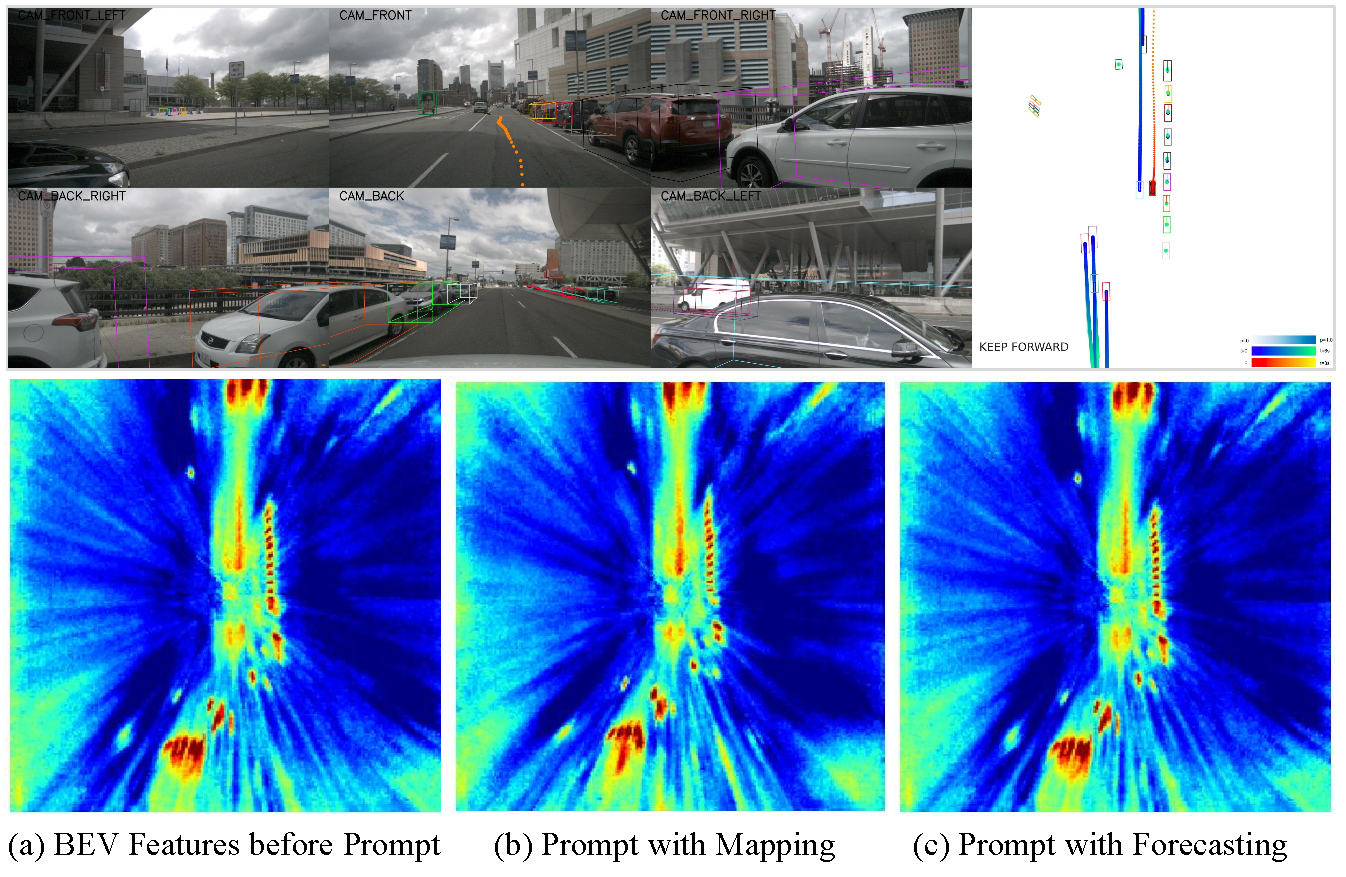
\includegraphics[width=0.45\textwidth]{figures/task} 
	\caption{Visualization of BEV feature maps when prompting with different tasks.}
	\label{fig:task}
\end{figure}

The nuScenes dataset~\cite{nuscenes} is a large-scale autonomous driving dataset that consists of 700, 150, and 150 sequences for training, validation, and testing, respectively. The scenes are recorded in Boston and Singapore, encompassing a diverse array of weather and lighting conditions, as well as various traffic scenarios.

The OpenScene dataset~\cite{openscene} is the largest 3D occupancy dataset, covering a wide span of over 120 hours of occupancy labels collected in various cities, from Boston, Pittsburgh, Las Vegas to Singapore. OpenScene provides a semantic label for each foreground grid and incorporates the motion information of occupancy flow that helps bridge the gap between decision-making and scene representation. we utilize both semantic occupancy labels and occupancy flow for the supervision of 4D pre-training. 

The dense 3D occupancy ground truth is derived by fusing multiple frames of LiDAR point clouds~\cite{occnet,uniscene}. This approach offers a more comprehensive representation of objects, encompassing details about occluded areas, in contrast to single-frame point clouds. In the future, it may become feasible to directly reconstruct 3D occupancy ground truth from autonomous driving videos using techniques such as NeRF~\cite{nerf,nerf2}, 3D Gaussian Splatting~\cite{3dgs}, and MVS~\cite{mvsnet,bi,aa-rmvsnet}.

\section{Task Prompt}
\begin{figure}[t]
	\centering
	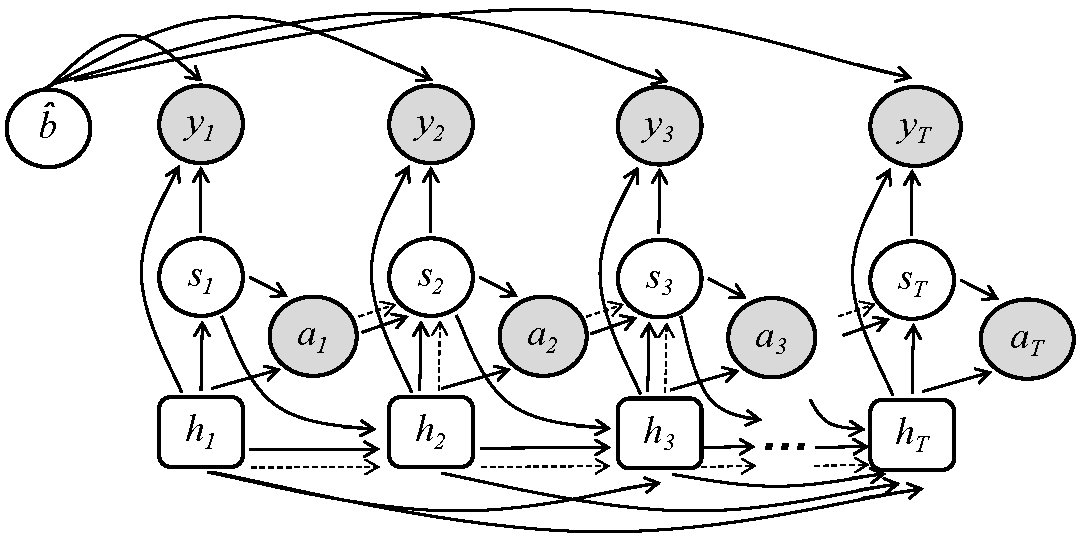
\includegraphics[width=0.45\textwidth]{figures/graph} 
	\caption{Graphical model of Memory State-Space Model. Deterministic states are denoted by squares, while stochastic states are represented by circles. The observed states are highlighted in grey for clarity. Solid lines represent the generative model, while dotted lines depict variational inference.}
	\label{fig:graph}
\end{figure}
\begin{figure*}[t]
	\centering
	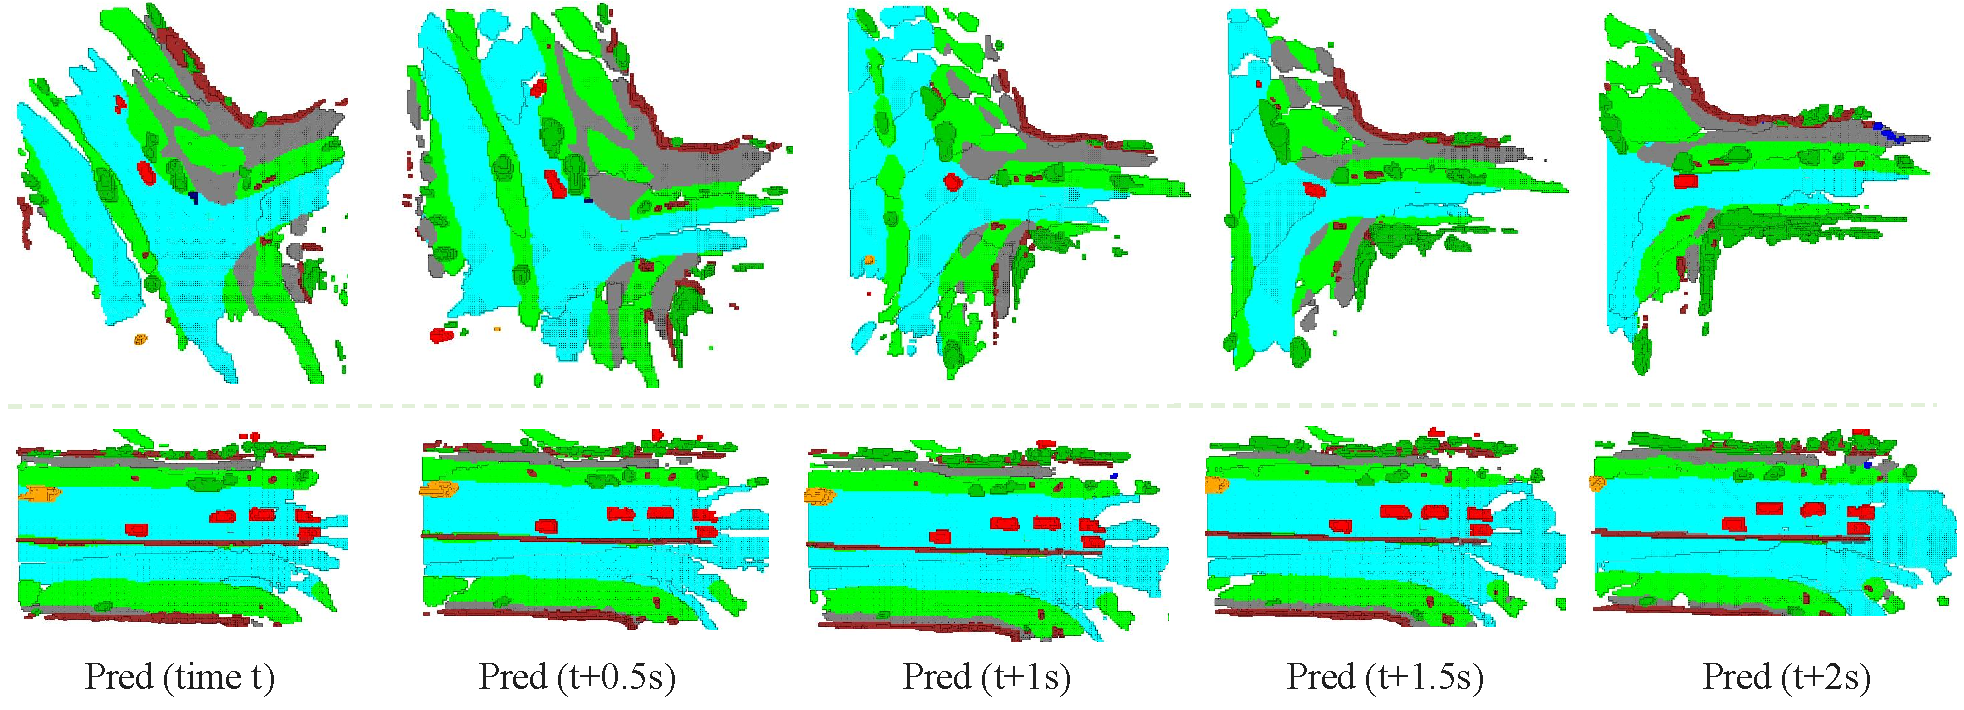
\includegraphics[width=0.99\textwidth]{figures/occ} 
	\caption{ Qualitative example of 3D occupancy predictions, for 2 seconds in the future.}
	\label{fig:show}
\end{figure*}
During fine-tuning, we add task prompts to BEV maps before each downstream task's decoder. For 3D object detection, the task prompt is ``The task is for 3D object detection of the current scene." For planning, the task prompt is ``The task involves planning with consideration for both the current and future scenes." The encoder network of task prompts is transferred to downstream tasks, and fine-tuning includes downstream task prompts. This enables different downstream tasks with semantic connections to decouple task-aware features. 
While basic embeddings for specific tasks are optional, large language model captures complex semantic relationships, providing a nuanced representation of task prompts. Additionally, the strong generalization abilities of such models enhance performance across a wide array of tasks when needed.
However, it's worth noting that the current Task Prompt design is relatively simple, and the task number for autonomous driving is limited.

In Fig.~\ref{fig:task}, we present visualizations of BEV feature maps both before and after the integration of various task prompts. 
Notably, as shown in Fig.~\ref{fig:task} (a), the BEV feature map based on 4D pre-training captures abundant information from both the current and future scenes. While, for specific downstream tasks, some information could be redundant or even detrimental. We utilize task prompts to alleviate the effect of redundant information.
In online mapping tasks, the feature map, guided by the task prompt, emphasizes the current spatio-aware information. The targets has more accurate location information in feature map to achieve higher precision .
For motion forecasting task, the feature map, guided by the task prompt, conserves both spatial and temporal information. The targets cover a broader region in feature map to achieve more robust prediction.

\section{Differences between RSSM and MSSM}
In world model-based methods such as Dreamers~\cite{dreamerv1, dreamerv2, dreamerv3} and MILE~\cite{mile}, the RSSM~\cite{latent} is commonly employed to learn latent variables. However, RSSM, relying on RNN networks, may encounter challenges related to long-term information retention. In contrast, our designed Dynamics Memory Bank in MSSM excels in modelling and preserving long-term information. RSSM compresses features into 1D tensor, while MSSM utilizes context BEV features to reconstruct 3D scenes. Besides, MSSM separates dynamic and static information, addressing them independently.

\section{Graphical Model}

In Fig.~\ref{fig:graph}, we illustrate the graphical model of the proposed Memory State-Space Model. The update of the deterministic state $h_t$ is dependent on the historical states in Dynamics Memory Bank, facilitating the transmission of temporal-aware features. Spatial-aware features are preserved through the retention of BEV feature $\hat{b}$. 

\section{Qualitative Results}

Fig.~\ref{fig:show} presents the reconstruction of both the current and future 3D scenes. This visual representation effectively illustrates DriveWorld's capacity for reconstructing the 3D scene and predicting future changes, thus enhancing downstream task performance after 4D pre-training.